% =====================================================================
%  CIT: 404 — RECOVERY PROTOCOL  ·  OPERATOR MANUAL  v2
%  Compile with: xelatex (twice for TOC page numbers)
%  Cover  : CIT 404 event poster full-page
%  Inner  : dimmed hacker/circuit image, green-accented text
% =====================================================================
\documentclass[11pt]{article}

\usepackage{fontspec}
\usepackage[a4paper,margin=20mm,top=22mm,bottom=22mm]{geometry}
\usepackage[dvipsnames]{xcolor}
\usepackage{tikz}
\usepackage{eso-pic}
\usepackage[most]{tcolorbox}
\usepackage{titlesec}
\usepackage{enumitem}
\usepackage{fancyhdr}
\usepackage{hyperref}
\usepackage{graphicx}
\usepackage{ragged2e}
\usepackage{atbegshi}

% ---------------------------------------------------------------------
%  PALETTE
% ---------------------------------------------------------------------
\definecolor{void}{HTML}{050505}
\definecolor{panel}{HTML}{0B0E0B}
\definecolor{edge}{HTML}{2A2A2A}
\definecolor{term}{HTML}{00FF41}
\definecolor{termdim}{HTML}{00B32D}
\definecolor{termfaint}{HTML}{0A3D17}
\definecolor{alert}{HTML}{FF003C}
\definecolor{warn}{HTML}{FFB000}
\definecolor{info}{HTML}{00E5FF}
\definecolor{item}{HTML}{FF4FA3}

% ---------------------------------------------------------------------
%  FONTS
% ---------------------------------------------------------------------
\setmainfont{JetBrainsMonoNerdFont-}[
  Path           = /usr/share/fonts/TTF/,
  Extension      = .ttf,
  UprightFont    = *Regular,
  BoldFont       = *Bold,
  ItalicFont     = *Italic,
  BoldItalicFont = *BoldItalic
]
\newfontfamily\displayfont{JetBrainsMonoNerdFont-}[
  Path        = /usr/share/fonts/TTF/,
  Extension   = .ttf,
  UprightFont = *ExtraBold,
  BoldFont    = *ExtraBold
]
\newcommand{\tracked}[1]{{\addfontfeatures{LetterSpace=14.0}#1}}
\newcommand{\trackedwide}[1]{{\addfontfeatures{LetterSpace=24.0}#1}}

% ---------------------------------------------------------------------
%  BACKGROUND MANAGEMENT
%  Cover (page 1) gets the full poster.
%  All other pages get the dimmed hacker image.
% ---------------------------------------------------------------------
\pagecolor{void}

% inner page background — dimmed hacker image, centred, fills the page
\newcommand{\innerbg}{%
  \AddToShipoutPictureBG*{%
    \begin{tikzpicture}[remember picture, overlay]
      \node[at=(current page.center), opacity=0.55] {%
        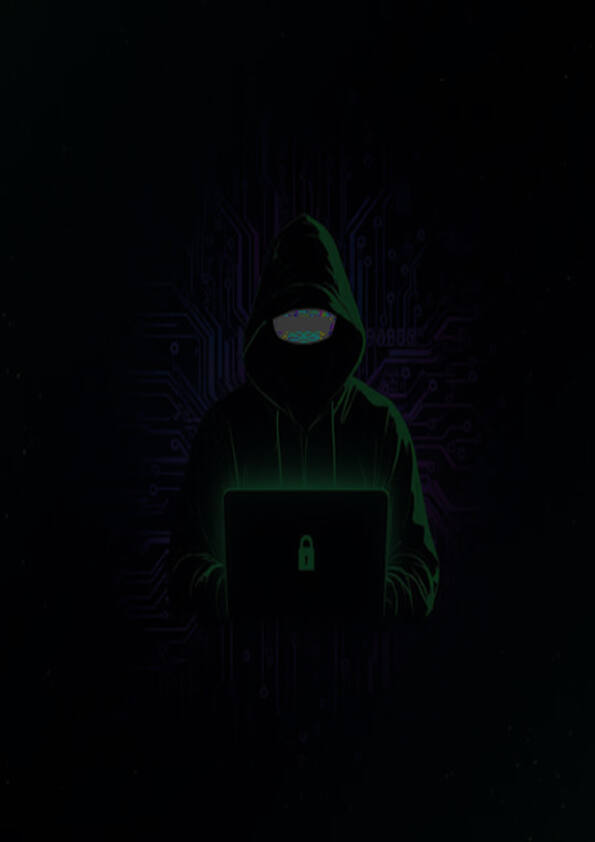
\includegraphics[width=\paperwidth,height=\paperheight,keepaspectratio=false]{bg_inner.jpg}%
      };
      % semi-transparent void overlay to push contrast back up
      \fill[void,opacity=0.45] (current page.south west) rectangle (current page.north east);
    \end{tikzpicture}%
  }%
}

\AtBeginDocument{\color{term!90}}

% ---------------------------------------------------------------------
%  LINKS
% ---------------------------------------------------------------------
\hypersetup{
  colorlinks=true, linkcolor=info, urlcolor=info,
  pdftitle={CIT: 404 — Recovery Protocol · Operator Manual},
  pdfauthor={CIT Club INPT}
}

% ---------------------------------------------------------------------
%  TCOLORBOX STYLES
% ---------------------------------------------------------------------
\newtcolorbox{mypanel}[1][]{
  enhanced, breakable,
  colback=black!70, colframe=edge, boxrule=0.5pt, sharp corners,
  left=4mm, right=4mm, top=3mm, bottom=3mm,
  overlay={
    \draw[term!80,line width=0.8pt]
      ([yshift=-2.5mm]frame.north west)--(frame.north west)--([xshift=2.5mm]frame.north west);
    \draw[term!80,line width=0.8pt]
      ([yshift=2.5mm]frame.south east)--(frame.south east)--([xshift=-2.5mm]frame.south east);
  }, #1
}
\newtcolorbox{terminal}{
  enhanced, breakable, colback=black!80, colframe=term,
  boxrule=0pt, leftrule=2pt, sharp corners,
  left=4mm, right=4mm, top=2.5mm, bottom=2.5mm,
  fontupper=\small
}
\newtcolorbox{alertbox}[1]{
  enhanced, breakable, colback=alert!12, colframe=alert,
  boxrule=1.2pt, sharp corners, left=4mm,right=4mm,top=3mm,bottom=3mm,
  fonttitle=\bfseries\displayfont\color{void},
  coltitle=void, attach boxed title to top left={yshift=-2mm,xshift=4mm},
  boxed title style={colback=alert,sharp corners,boxrule=0pt},
  title={\tracked{#1}}
}
\newtcolorbox{warnbox}[1]{
  enhanced, breakable, colback=warn!10, colframe=warn,
  boxrule=1.2pt, sharp corners, left=4mm,right=4mm,top=3mm,bottom=3mm,
  fonttitle=\bfseries\displayfont\color{void},
  coltitle=void, attach boxed title to top left={yshift=-2mm,xshift=4mm},
  boxed title style={colback=warn,sharp corners,boxrule=0pt},
  title={\tracked{#1}}
}
\newtcolorbox{infobox}[1]{
  enhanced, breakable, colback=info!8, colframe=info,
  boxrule=1.2pt, sharp corners, left=4mm,right=4mm,top=3mm,bottom=3mm,
  fonttitle=\bfseries\displayfont\color{void},
  coltitle=void, attach boxed title to top left={yshift=-2mm,xshift=4mm},
  boxed title style={colback=info,sharp corners,boxrule=0pt},
  title={\tracked{#1}}
}

% ---------------------------------------------------------------------
%  HEADINGS
% ---------------------------------------------------------------------
\newcommand{\secfmt}[1]{\tracked{\MakeUppercase{#1}}}
\titleformat{\section}
  {\displayfont\Large\color{term}}
  {\color{termdim}\texttt{>\,}\colorbox{termfaint}{\color{term}\,\thesection\,}}
  {0.8em}{\secfmt}
  [{\vspace{-0.4em}\color{termfaint}\rule{\linewidth}{0.5pt}}]
\titleformat{\subsection}
  {\displayfont\normalsize\color{warn}}
  {\color{warn}\texttt{::}}{0.6em}{\secfmt}
\setlength{\parskip}{0pt}
\titlespacing*{\section}{0pt}{1.6em}{0.8em}
\titlespacing*{\subsection}{0pt}{1.0em}{0.4em}

% ---------------------------------------------------------------------
%  HEADER / FOOTER  (inner pages only)
% ---------------------------------------------------------------------
\pagestyle{fancy}\fancyhf{}
\renewcommand{\headrulewidth}{0.4pt}
\renewcommand{\footrulewidth}{0.4pt}
\renewcommand{\headrule}{\hbox to\headwidth{\color{termfaint}\leaders\hrule height\headrulewidth\hfill}}
\renewcommand{\footrule}{\hbox to\headwidth{\color{termfaint}\leaders\hrule height\footrulewidth\hfill}}
\fancyhead[L]{\footnotesize\color{term!60}\texttt{CIT:404}}
\fancyhead[R]{\footnotesize\color{term!60}\texttt{RECOVERY\_PROTOCOL}}
\fancyfoot[L]{\footnotesize\color{term!45}\texttt{// OPERATOR MANUAL}}
\fancyfoot[C]{\footnotesize\color{term!45}\texttt{CIT CLUB INPT}}
\fancyfoot[R]{\footnotesize\color{term!60}\texttt{\thepage}}

\setlist[itemize]{leftmargin=1.4em,itemsep=2pt,topsep=3pt,label={\color{term}\texttt{>}}}
\setlist[enumerate]{leftmargin=1.6em,itemsep=2pt,topsep=3pt}

\newcommand{\chip}[2]{{\setlength{\fboxsep}{2pt}\colorbox{#1!18}{\color{#1}\footnotesize\textbf{\texttt{#2}}}}}
\newcommand{\cit}{\textbf{\color{warn}CIT\$}}
\newcommand{\nrg}{\textbf{\color{info}Core Energy}}

% =====================================================================
\begin{document}
\RaggedRight

% =====================================================================
%  COVER PAGE — full event poster, no header/footer
% =====================================================================
\thispagestyle{empty}
\newgeometry{margin=0pt}
\begin{tikzpicture}[remember picture, overlay]
  \node[at=(current page.center)] {%
    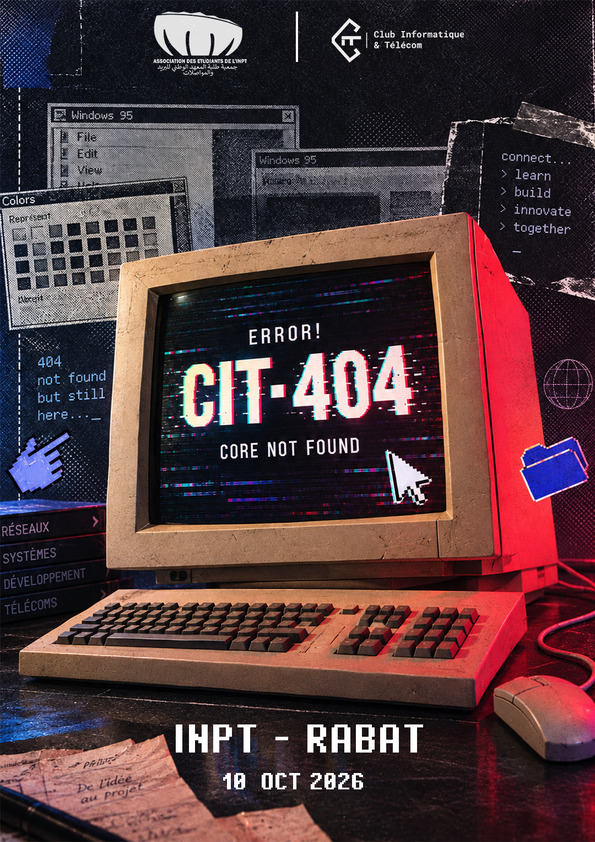
\includegraphics[width=\paperwidth,height=\paperheight,keepaspectratio=false]{bg_cover.jpg}%
  };
  % light dark vignette at bottom for the footer text
  \fill[void,opacity=0.55]
    (current page.south west) rectangle
    ([yshift=38mm]current page.south east);
\end{tikzpicture}%
% Footer text over poster
\vspace*{\fill}
\begin{center}
  {\color{term!40}\footnotesize\texttt{CLASSIFIED // FOR RECRUITED OPERATORS ONLY // DO NOT DISTRIBUTE}}
\end{center}
\restoregeometry
\clearpage

% =====================================================================
%  INDEX PAGE
% =====================================================================
% Apply hacker background persistently to ALL pages from here onward
\AddToShipoutPictureBG{%
  \begin{tikzpicture}[remember picture, overlay]
    \node[at=(current page.center), opacity=0.55] {%
      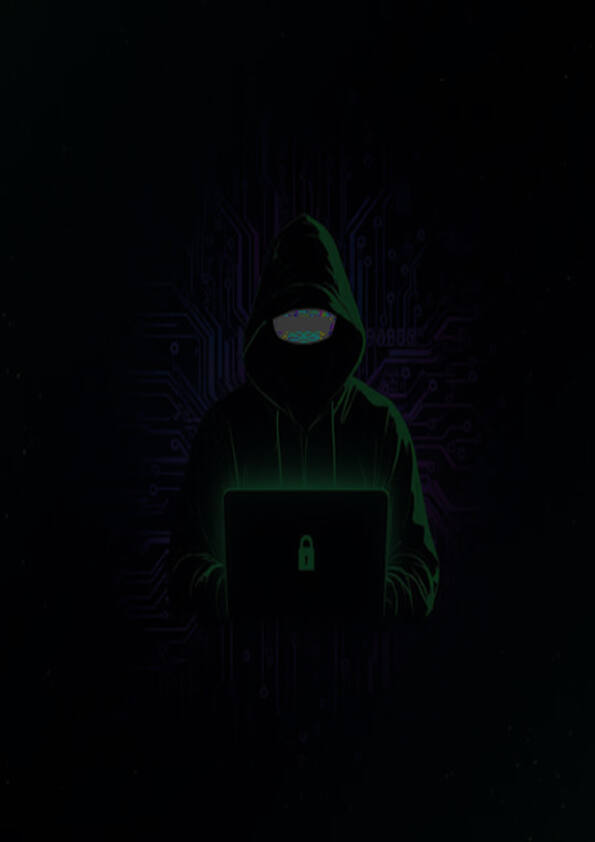
\includegraphics[width=\paperwidth,height=\paperheight,keepaspectratio=false]{bg_inner.jpg}%
    };
    \fill[void,opacity=0.45] (current page.south west) rectangle (current page.north east);
  \end{tikzpicture}%
}
{\displayfont\Large\color{term}\tracked{SYSTEM INDEX}}\\[-0.3em]
{\color{termfaint}\rule{\linewidth}{0.5pt}}
\vspace{0.4em}
\renewcommand{\contentsname}{}
\makeatletter\@starttoc{toc}\makeatother
\clearpage

% =====================================================================
\section{Incoming Transmission}
% =====================================================================
\begin{terminal}
\color{term!85}
\texttt{> SYSTEM FAILURE DETECTED.}\\
\texttt{> NETWORK STABILITY: 0\%.}\\
\texttt{> RECOVERY PROTOCOL ACTIVATED.}\\
\texttt{\color{term}> NEW OPERATORS REQUIRED.}
\end{terminal}

\vspace{0.5em}
Year 2026. For years the CIT Network ran quietly in the background —
connecting knowledge, technology, intelligence and innovation through one
central system known only as \textbf{THE CORE}.

At 09:00 the network detected an unknown anomaly. At 09:01 systems began
shutting down. At 09:03 communication between sectors was lost.
\textbf{\color{alert}At 09:05, THE CORE went offline.}

The network collapsed. Its core systems are dark. You and your teammates
have been recruited as \textbf{Operators} — the people trusted to bring it
back. To restore the network you will earn resources, recover lost data, and
complete missions out in the real world.

This manual is your briefing. Read it once before the event and you will know
everything you need. Nothing here reveals the puzzles themselves — only how
the protocol works.

\begin{infobox}{NO EXPERIENCE REQUIRED}
If you have never touched a line of code or played anything like this before:
\textbf{good — you belong here.} CIT:404 is built for complete beginners.
Every phase has an easy entry point, your teammates cover each other's weak
spots, and you can buy help whenever you are stuck. You are not expected to
know anything in advance. Be curious, talk to your team, and try. That is the
whole job.
\end{infobox}

% =====================================================================
\section{Your Squad}
% =====================================================================
You play as a \textbf{team of three Operators} sharing a single account.

\begin{mypanel}
\begin{itemize}
  \item \textbf{One team, one wallet.} The three of you share the same balance,
        inventory and progress. Money one operator earns is instantly available
        to the others.
  \item \textbf{Each person has a callsign.} When you log in, type your own
        nickname — it just records who did what so your team can see who solved
        a challenge or spent the money.
  \item \textbf{One shared access code.} Your team receives a single join code.
        All three operators enter the same code to connect.
\end{itemize}
\end{mypanel}

\subsection{Connecting to the Network}
\begin{enumerate}
  \item Open the platform link the organizers give you (any phone browser works).
  \item Choose your \textbf{team}, type \textbf{your callsign}, enter the
        \textbf{team access code}.
  \item You are in. If you refresh or your phone sleeps, the session restores
        automatically — you will not be kicked out mid-game.
\end{enumerate}

\begin{warnbox}{KEEP YOUR CODE SAFE}
Your team access code is the key to your wallet. Do not hand it to another
team. If a device is lost, tell an admin — they can disconnect that one device
without logging the rest of your team out.
\end{warnbox}

\clearpage
% =====================================================================
\section{The Economy}
% =====================================================================
Everything in CIT:404 runs on two resources. Watch both.

\begin{mypanel}
\textbf{\cit{}} — your \textbf{currency}. Earn it by solving challenges and
completing missions, spend it in The Market on help and advantages.
\\[6pt]
\textbf{\nrg{}} — your \textbf{restoration score}. It measures how much of the
network you have brought back. Energy is what the leaderboard ranks you on —
it is effectively your \textbf{score}.
\end{mypanel}

\subsection{First Blood}
The \textbf{first team} to solve a given challenge earns a one-time
\textbf{First Blood} bonus — extra \cit{} and \nrg{} on top of the normal
reward. It pays to be fast, but every team that cracks a challenge still gets
paid. First Blood is decided by the server; ties cannot produce two winners.

\subsection{The Market}
Stuck? Spend \cit{} on help instead of burning time. The Market sells:
\begin{itemize}
  \item \chip{warn}{HINTS} — nudges and partial solutions when you are stuck.
  \item \chip{info}{INSURANCE} — protects your investment if a mission fails.
  \item \chip{item}{BOOSTS} — advantages that change how a mission plays out.
  \item \chip{term}{ACCESS} — unlock extra information or routes.
\end{itemize}
Everything you buy lands in your team's shared inventory, usable by all three
operators. Spending wisely is part of the game — knowledge has a price, and so
does wasting it.

\begin{infobox}{THE LEDGER NEVER LIES}
Every movement of \cit{} and \nrg{} is written to a permanent record your
team can view at any time. The Transaction Log names who spent what and when.
If something looks wrong, show an admin — disputes are settled from this record.
\end{infobox}

% =====================================================================
\section{The Three Phases}
% =====================================================================
The protocol runs in phases, and \textbf{only one phase is open at a time}.
The admins (THE CORE) decide when each one opens. Tabs for phases that are not
active appear locked — that is normal, your time will come.

\subsection{Phase I — Digital Arena}
The on-screen phase. You solve short challenges in three families. Each solve
pays \cit{} and \nrg{}. You submit answers in the form of a
\textbf{flag} — a short code that usually looks like \texttt{CIT\{...\}}.
Find the flag, type it in, get paid.

\begin{mypanel}
\textbf{\color{term}CP — Computational Problems.}\\
Logic and reasoning puzzles. Work out the answer from a description. The easy
ones require pure thinking — no heavy programming needed to start.
\\[6pt]
\textbf{\color{info}CTF — Capture The Flag.}\\
Something is hidden and your job is to find it. Look where most people do not:
inside pages, files, messages. The flag is waiting to be uncovered.
\\[6pt]
\textbf{\color{warn}DATA — Data Challenges.}\\
You are given information — logs, records, fragments — and asked a question.
The answer is in the data; you just have to read it the right way.
\end{mypanel}

\begin{infobox}{HOW A BEGINNER WINS PHASE I}
Split the three families between the three of you and shout out what you find.
Start with the one-star challenges — they are designed for someone seeing this
for the first time. If you stall for more than a few minutes, \textbf{buy a
hint}. A cheap hint that unblocks you is almost always worth more than the
\cit{} it costs.
\end{infobox}

\subsection{Phase II — Field Operations}
This phase leaves the screen. Missions send your team out into the real world
to complete tasks. The flow is simple:

\begin{enumerate}
  \item \textbf{Read the intel.} Each mission gives you a clue about a location.
        Work out where it points and go there.
  \item \textbf{Get the code on site.} Once you physically reach the location,
        an admin gives you an access code that unlocks the mission. (You can
        also spend an item to reveal exact coordinates.)
  \item \textbf{Choose your difficulty.} Each mission offers
        \chip{term}{EASY} / \chip{warn}{MEDIUM} / \chip{alert}{HARD}. Harder
        tiers cost more \cit{} and pay more \cit{} and \nrg{}. Pick what your
        team can actually pull off.
  \item \textbf{Complete the task and prove it.} An admin validates your proof
        on site and your reward lands in the wallet.
\end{enumerate}

There is also a free \textbf{Supply Run} for teams who run out of \cit{} — a
no-cost mission so nobody gets permanently stuck.

\begin{alertbox}{FIELD CONDUCT — THIS IS NOT OPTIONAL}
Field missions involve real people and real public space. Operators who break
these rules can be penalized or disqualified:
\begin{itemize}
  \item \textbf{Always ask consent} before photographing, filming or recording
        anyone. If a person says no, thank them and move on.
  \item \textbf{Be respectful and polite.} You represent CIT Club and INPT.
        No harassment, no pressure, no blocking people's way.
  \item \textbf{Stay safe.} Watch traffic, do not trespass, do not enter
        restricted or private areas, and stay with your team.
  \item \textbf{Nobody is forced to participate.} Members of the public are
        bystanders, not players.
\end{itemize}
\end{alertbox}

\subsection{Phase III — Endgame}
The final phase. The truth about THE CORE is broken into \textbf{six
fragments}, each locked behind a code you earn from the admins. Recover a
fragment and you are paid in \cit{} and \nrg{} — and you receive a piece of
the story. Assemble all six and you learn what really happened the day the
network fell.

\begin{terminal}
\color{term!80}
\texttt{> FRAGMENTS RECOVERED: 0 / 6}\\
\texttt{> STORY INTEGRITY: INCOMPLETE}\\
\color{alert}\texttt{> DID YOU RESTORE THE SYSTEM... OR DID YOU JUST SET IT FREE?}
\end{terminal}

\clearpage
% =====================================================================
\section{Orders From The Core}
During the event the admins can send your team messages directly.

\begin{mypanel}
\textbf{\color{info}Normal transmissions} arrive in your messages panel.
They are information — read them when you like.\\[6pt]
\textbf{\color{alert}Urgent orders} take over your whole screen with a red
countdown. You \emph{must} acknowledge them. Completing the order in time pays
a reward; letting the timer run out costs you \cit{} and \nrg{}
\textbf{automatically} — even if you closed the tab. Acknowledging an order is
not the same as completing it; an admin confirms the real outcome.
\end{mypanel}

\begin{warnbox}{WHEN THE SCREEN GOES RED}
Stop, read the order, and act. The countdown is real and the penalty is
automatic. Do not ignore an urgent order hoping it goes away — it will not.
\end{warnbox}

% =====================================================================
\section{The Leaderboard}
% =====================================================================
Standings are live and visible to every team. Teams are ranked by \nrg{}
(your restoration score), with total \cit{} earned as the tie-breaker.
Solve challenges, complete missions, grab First Bloods and recover fragments —
all of it feeds your rank. The board updates in real time, so a strong final
push genuinely changes the outcome.

% =====================================================================
\section{Operator Code of Conduct}
% =====================================================================
\begin{mypanel}
\begin{itemize}
  \item \textbf{Play your own game.} Do not share answers, flags or codes with
        other teams, and do not take theirs.
  \item \textbf{Stay in scope.} Solve the challenges as designed. Do not attack
        the platform, the network, or the organizers' infrastructure — that is
        not part of the game and ends your event immediately.
  \item \textbf{Respect people and place.} Field-conduct rules apply all day,
        everywhere.
  \item \textbf{Help your teammates.} Three beginners who talk to each other
        beat one expert who goes silent. Every time.
  \item \textbf{Ask the admins.} Stuck, confused, or something looks broken?
        Find an organizer. They would rather help than watch you struggle.
\end{itemize}
\end{mypanel}

\vspace{0.5em}

% =====================================================================
%  OUTRO PAGE — deliberately centred on the hacker background
% =====================================================================
\clearpage
\thispagestyle{fancy}
\vspace*{\fill}
\begin{center}
\begin{tcolorbox}[enhanced, width=0.88\linewidth,
  colback=black!80, colframe=term, boxrule=1pt, sharp corners,
  halign=center,
  overlay={
    \draw[term,line width=1.2pt]
      ([yshift=-4mm]frame.north west)--(frame.north west)--([xshift=4mm]frame.north west);
    \draw[term,line width=1.2pt]
      ([yshift=4mm]frame.south east)--(frame.south east)--([xshift=-4mm]frame.south east);
    \draw[term!40,line width=0.6pt]
      ([yshift=-4mm]frame.north east)--(frame.north east)--([xshift=-4mm]frame.north east);
    \draw[term!40,line width=0.6pt]
      ([yshift=4mm]frame.south west)--(frame.south west)--([xshift=4mm]frame.south west);
  }]
  \vspace{0.3em}
  {\displayfont\Large\color{term}\trackedwide{CIT:404}}\\[4pt]
  {\color{alert}\small\tracked{THE CORE HAS FALLEN}}\\[12pt]
  {\displayfont\normalsize\color{term}\tracked{THE NETWORK IS WAITING, OPERATOR.}}\\[6pt]
  {\color{term!70}\small Earn.\ \ \ Recover.\ \ \ Restore.}
  \quad{\color{alert}\small Or set it free.}\\[14pt]
  
\includegraphics[width=3.5cm]{logo_white.png}\\[6pt]
  {\color{term!40}\footnotesize\texttt{CIT CLUB INPT \ // \ INPT RABAT IRFANE \ // \ 10.10.2026}}
  \vspace{0.3em}
\end{tcolorbox}
\end{center}
\vspace*{\fill}

\end{document}
